\section{Module}
\label{subs:module}
Since a configuration is made up of individual modules, it seems natural to model it as a set of communicating module instances. By observing the FESTO CP-Learning Factory setup at Aalborg university, we chalk up the following  module characteristics:

\begin{itemize}
\item Modules are square or rectangle and have different physcial dimensions.
\item Several types of work may be performed by the same module. \checkmark
\item An item may pass through a module without have work performed on it. \checkmark
\item Items queue up in a module and wait to be processed or just pass through. \checkmark
\item Some modules allow for items to pass through while processing another item. Others do not. \checkmark
\item A module may employ a seperate queue to store items that it is going to work on. 
\item Some modules are only used for transport. \checkmark
\item The time taken to transport an item over a module, depends on where the item enters and leaves. \checkmark
\item An item may leave a module from any of its four sides, if there is another module ready to accept it. \checkmark
\end{itemize} 

On the list above, checkmarks indicate which characteristics we have chosen to implement directly in our model. While these observations were made from a specific system, we feel that they are general enough to apply to modular factories as a whole. 

The physcial apsect of  modules are not enforced in our model. Two modules can be connected and pass items between each other, even though this may not physically be possible. Later in \cref{ch:configuration} we show, how we enforce some rules of physicality, when generating configurations outside of UPPAAL. We do not implement seperate module queues for items that need to be worked on. This would not have been difficult to implement. Yet, we see it as an edge case that would add onto our state space. Thus we choose to disregard it. The rest of the chracteristics we choose to implement in our model in one way or the other.

\begin{figure}[h]
\centering
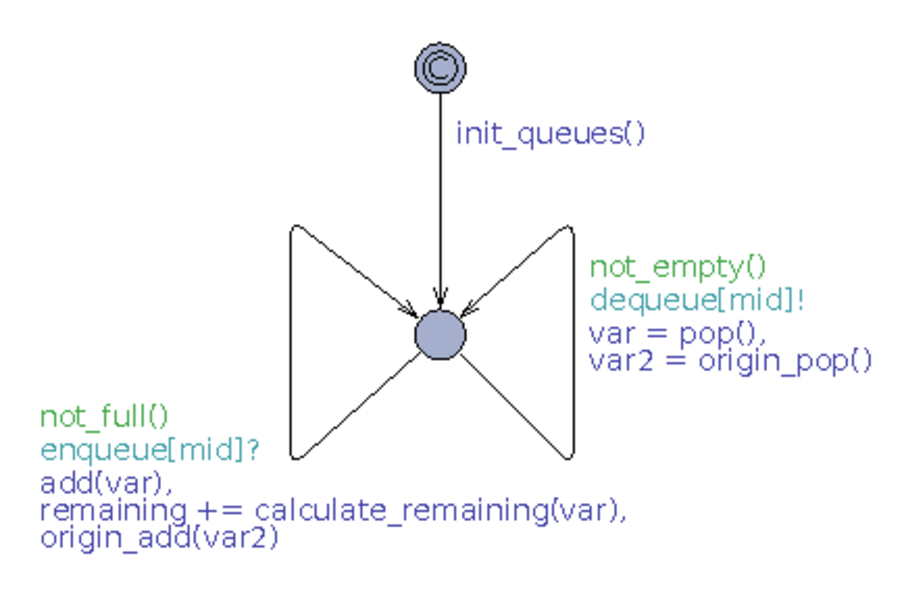
\includegraphics[width=\textwidth]{modulequeue.pdf}
\caption{The ModuleQueue template}
\label{fig:modulequeue}
\end{figure}

One of the most important observed characteristics was the queuing nature of the system. Several items may be located on a module, but only one is being processed at a time. Some of the items queued may need to be processed, others just want to be passed along to a neighbouring module. Based on this behavior we construct the \emph{ModuleQueue} template. One such queue is instanziated for each module, and has a fixed size of items it may hold. Other modules may be able to use the \emph{enqueue} channel to move an item onto the module. In addition items may be removed from it through a synchronization on its \emph{dequeue} channel. The later synchronization is done by the other parts of the module, which are instances of the \emph{ModuleWorker} template and the \emph{ModuleTransporter} template. In this way, a module is actually made up of three different instances sharing an identifier and communicating across the same channels.    


\begin{figure}[h]
\centering
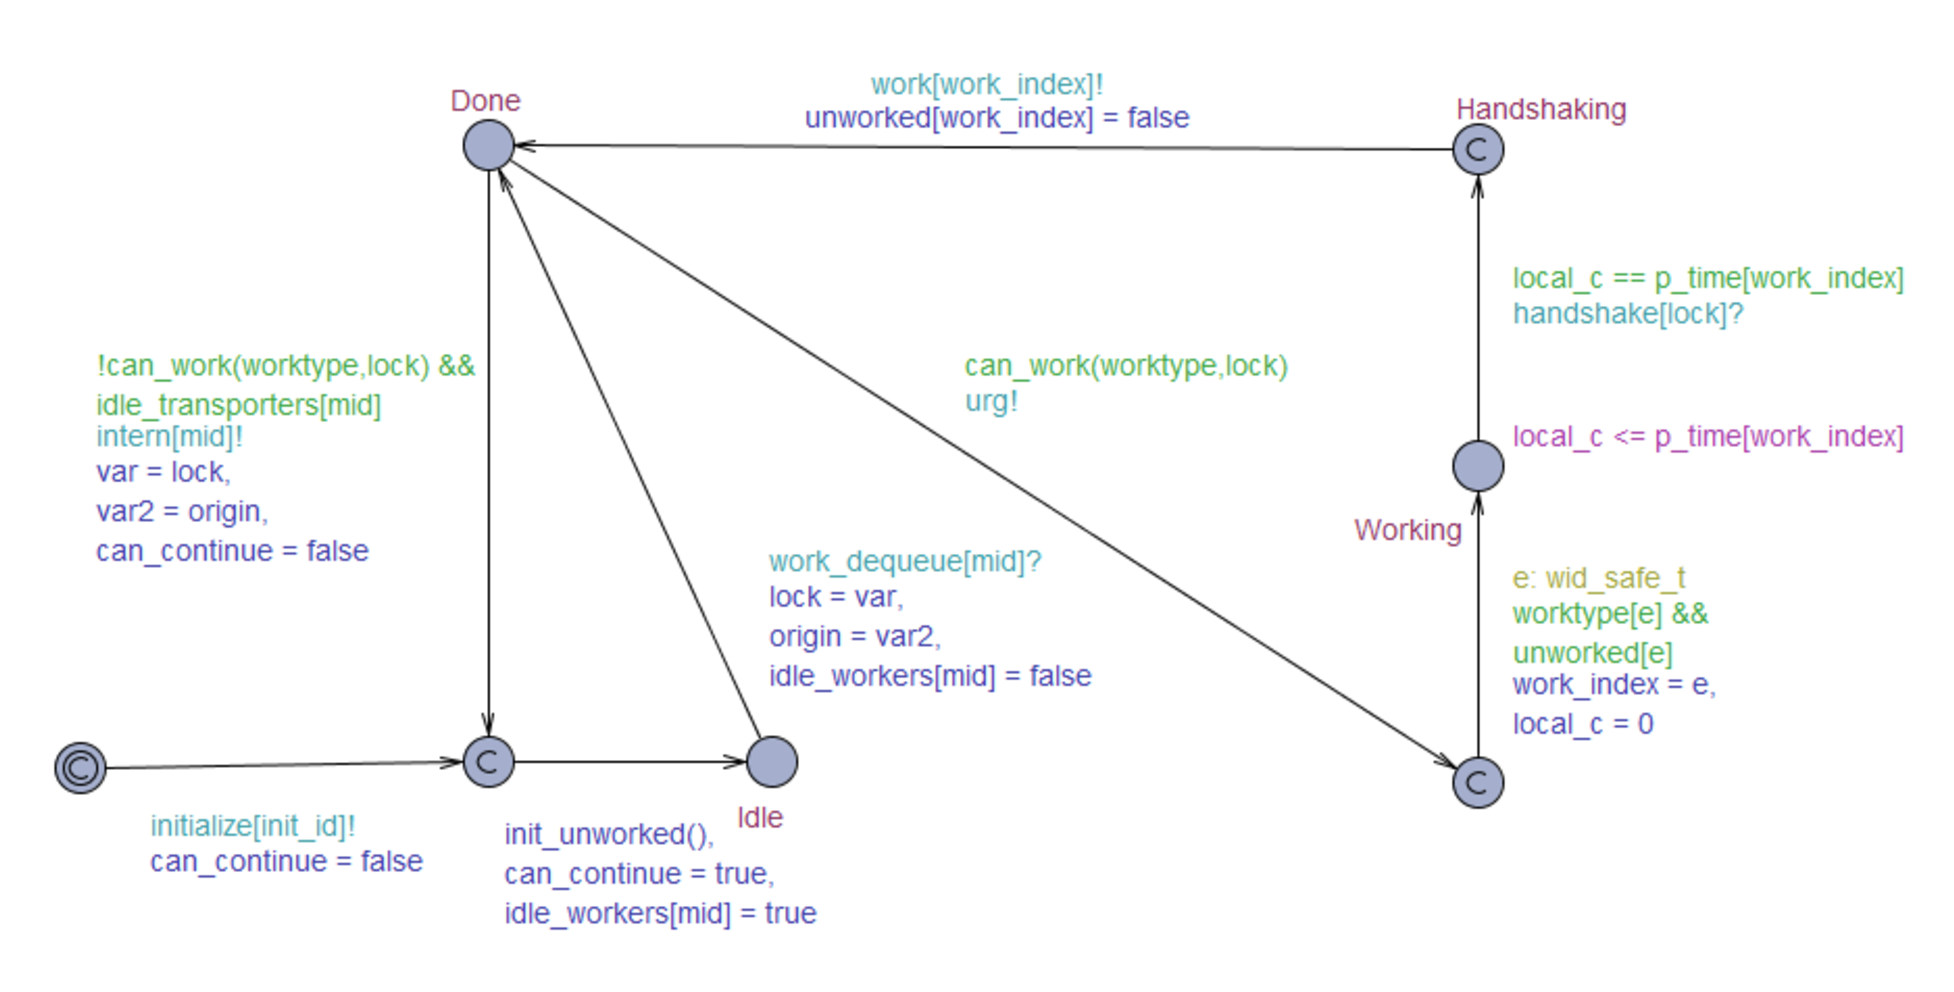
\includegraphics[width=\textwidth]{moduleworker.pdf}
\caption{The ModuleWorker template}
\label{fig:moduleworker}
\end{figure}

The \emph{ModuleWorker} template can be seen in \cref{fig:moduleworker}. An instance of this template performs the processing a module performs upon a recipe. It may apply several different types of work upon a recipe in succession before sending it the module's \emph{ModuleTransporter} instance. In the idle location, the worker waits to synchronize with the module's \emph{ModuleQueue} instance. Once this is done, it is passed the recipe's id through the global \emph{var1} variable. If the module can perform some work, it will move into the \emph{Working} location. Here it will wait for \emph{p\_time} and increment the global cost by \emph{cost\_rate}. When the wait is over, it will try to communicate with the recipe through the \emph{handshake} and \emph{work} channels as presented in \cref{sec:recipe}. Arriving at the \emph{Done} location, we may choose to work the recipe further if possible. Otherwise we perform a synchronization on the module's \emph{intern} channel. This passes the item over to the module's \emph{ModuleTransporter} instance.

The \emph{ModuleTransporter} template can be seen in \cref{fig:moduletransporter}. Using an instance of this template, a module may transport an item and pass it onto a neighbouring module. If the item comes from the module's \emph{ModuleWorker} instance, then we move into the \emph{Selector} location by synchronizing on the module's \emph{intern} channel. We may however also move directly to the \emph{Selector} location by synchronizing  with the module's \emph{ModuleQueue} instance over the \emph{dequeue} channel. However, this can only be done if the \cref{fig:moduletransporter} is instantiated with the local \emph{pass\_through} variable  set to \emph{True}. This boolean allows us to indicate, whether an item may be passed through the module or not, while another item is being processed by the module. This edge also allows us to create module's which only transport recipes. By not instantiating a module's \emph{ModuleWorker}, the only option for a recipe being transported into the module is to be passed on. 

Once in the \emph{Selector} location the recipe may go back to \emph{Idle} or \emph{Transporting}. If the recipe is done, it has to go back to idle and be removed from the production line by synchronizing on the \emph{remove} channel. If it is not done, it may look for a neighbouring module to be passed onto.  A module may have up to four neighbours, one on each side. These are stored in the local \emph{next} array, their index indicating their placement relative to the module. When moving to \emph{Transporting} location, the recipe will choose a possible neighbour. In \emph{Transporting} we wait to simulate the time taken to transport a recipe over the module. This time varies according to where the recipe enters the module, and where it leaves. The different transport times are stored in the 4 by 4 multidimensional \emph{t\_time} array. Given that we at this point know the side which the recipe entered from \emph{origin} and the side on which it will leave \emph{succ}, we can look up the exact time to wait in \emph{t\_time}. Once the wait is over we synchronize with the neighbour module's \emph{ModuleQueue} instance on the \emph{enqueue} channel. At the same time we use the local \emph{inverse} function to calculate from which side the recipe enters the neighbouring module. This is sent along with the global \emph{var2} variable and is later saved into the neighbour's \emph{origin} variable. 


\begin{figure}[h]
\centering
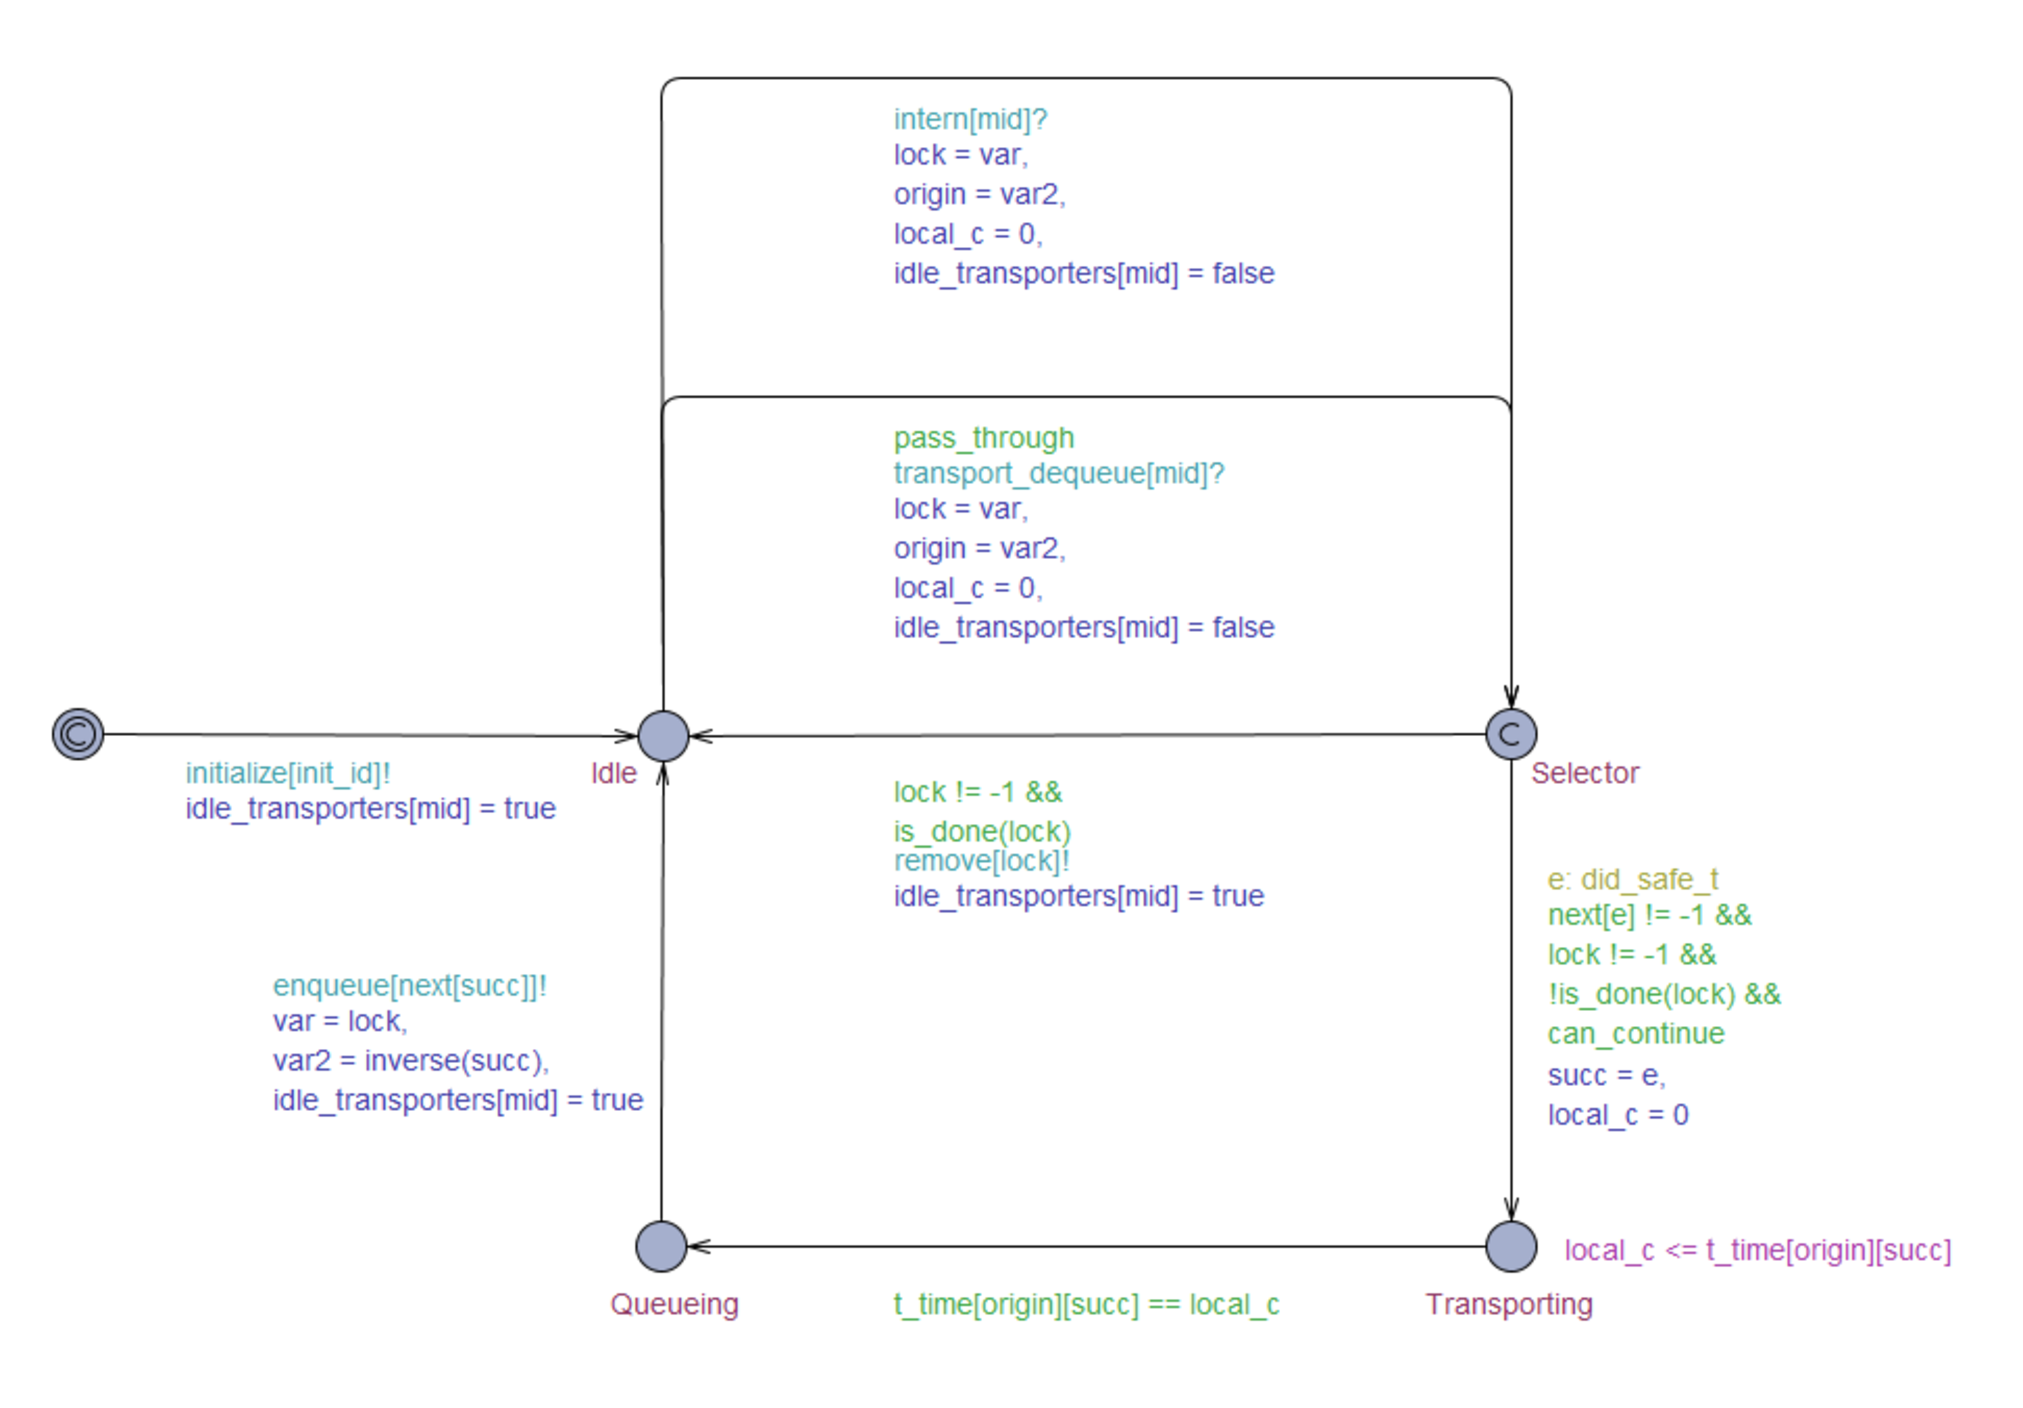
\includegraphics[width=\textwidth]{moduletransporter.pdf}
\caption{The ModuleTransporter template}
\label{fig:moduletransporter}
\end{figure}